\section{Introduction}
\label{section_intro}

\begin{figure}
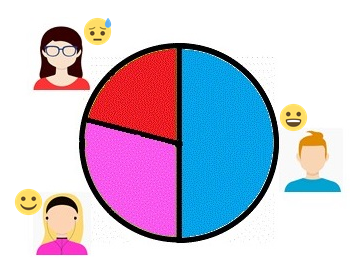
\includegraphics[width=2in]{images/cake_cutting.png}\Description{Cake-cutting Problem}
\caption{Fairness in cake cutting problem}
\end{figure}

Resource allocation has been one of the primary focus areas of economics since the beginning. It is also one of the most extensively studied one. The real-world is composed of limited resources as well as limited number of people who are going to use those resources. The problem of allocation of resources applies to both conditions in which, on one side, the resources are abundant (excess supply) or the other side where the number of users are larger (excess demand). Even with enough quantity of resources and consumers, each consumer may have different priority for different kinds of resources resulting in a complex allocation problem.

Two important concerns, among many others, in a resource allocation problem are efficiency and fairness. Efficiency criteria try to maximize the value that can be extracted from the available resources. Different types of efficiency criteria exist in resource allocation problem. One criterion may try to achieve the maximum possible value while other may try to optimize the utilization of all the available resources. We study some of these in greater details further in the paper. The fairness criterion tries to achieve overall welfare/goodness for all of the agents involved in the allocation problem. The idea of fairness have different perspectives depending upon the problem being studied. That may include equitability, where every agent gets an equal share in the allocation depending upon the agent's own subjective evaluation of the idea of equal share. Another interesting fairness perspective, which has gained much attention in the economics of fair allocation is envy-freeness. Envy-freeness ensures each agent prefers and values its own allocation more than the allocation of any other agent. We study this in more details in later sections.

The efficiency and fairness criteria are well studied for various types of goods in the market. One classification of such goods is based on divisibility. A divisible good, as the name suggests, can be described as the one which could be divided in fractions to achieve some form of allocation between multiple agents. Cake-cutting is a famous fair division problem with divisible goods. In cake-cutting problem, we need to divide a cake (or $m$ pieces of cakes) among some number of people in the party. \cite{varian1973equity} proposes competitive equilibrium for equal incomes (CEEI) for such a fair division problem. In CEEI, all agents are given equal income for fairness. Then each agent spends the income on some goods based on the agent's value for the good. In the cake division problem, a young individual may spend more to get a larger portion of the cake than an old person. The allocation is fair in terms of envy-freeness as each agent prefers its own allocation based on the value it has for that allocation. If it has more value, it will spend more to get larger fraction of the divisible good.

\begin{figure}
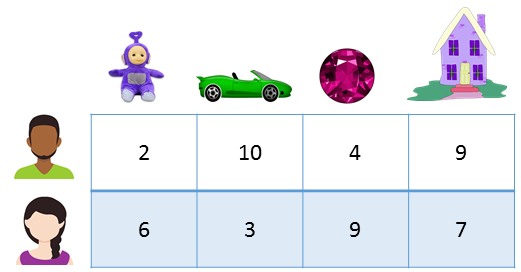
\includegraphics[width=3in]{images/indivisible_allocation2x4.png}\Description{Indivisible goods in Inheritance distribution}
\caption{Utilities of indivisible items in inheritance allocation}
\end{figure}

Introduction of indivisibility in goods takes away the envy-free property of the CEEI. More generally, envy-free solution does not exist for indivisible goods. Consider a simple resource allocation problem with one good and two agents. Since the good is indivisible, only one agent may get the object. The other agent will always envy for not getting the good. \cite{budish2011combinatorial} defines an approximation of the envy-freeness property for approximate-CEEI with indivisible goods. \cite{budish2011combinatorial} defines envy-freeness up to one good (EF1) as an approximation for envy-freeness and proves CEEI to be EF1 for additive utilities.

A welfare criteria we analyze in this paper is Nash social welfare. Nash social welfare is the product of values of allocations for each agent. An allocation which maximizes the Nash social welfare has interesting efficiency and fairness properties. The maximum Nash welfare (MNW) solution is envy-free for divisible goods. \cite{caragiannis2016unreasonable} shows MNW to provide efficient and fair solution even for divisible goods. An MNW solution for indivisible goods with additive utilities is guaranteed to be EF1 \cite{caragiannis2016unreasonable} with the same definition of EF1 defined by \cite{budish2011combinatorial}. Along with that, MNW solution is Pareto-optimal, hence uniquely demonstrating the elusive combination of both efficiency and fairness.

The MNW solution clearly seems to cater to both of the divisibility based classes of goods. But it assumes the additive nature of values that the agents have for various goods. This assumption hardly holds for the real world which is full of examples showing non-additive utilities of various forms. The EF1 fairness of MNW solution does not hold for non-additive goods. 

In this paper, we consider two such forms of non-additive goods: complementary goods and substitute goods. Complementary goods are the type of goods which show equivalent demand in market. If price for A increases, it's demand will decrease, decreasing the demand of another good B which is a complement of A. Substitute goods show an inverse behaviour. If price for A increases, its demand will decrease; while the demand for B which is A's substitute will increase. Both of these are well analyzed in economics and are used in the form of market strategies for increasing the overall utility and profit from a set of goods \cite{lewbel1985bundling, kojima1975international, bulow1985multimarket}. We relax the definition of envy-freeness up to one good (EF1) \cite{budish2011combinatorial} to introduce envy-freeness up to k goods (EFk). We analyze the efficiency and fairness of maximum Nash Welfare (MNW) for such goods and prove that MNW for such goods is bounded by EFk fairness criteria.

The rest of the paper is structured as follows. We study existing related research and topics in section \ref{section_related}. We introduce, define, and discuss terminologies and definitions in section \ref{section_prelim}. We analyze experimental results in section \ref{section_experiments}. Further, we analyze and formally prove EFk criteria for MNW allocation of complementary and substitute goods in section \ref{section_proof}. Finally, we conclude and discuss future directions in section \ref{section_conclusion}.

% End of section 1 ----------------------------------------------------------

\section{Related Work}
\label{section_related}
In this section, we will analyze the existing research on related topics.


\hrule
x
\hrule


\subsection{Network Embeddings}
Network provides a universal way to structure various real-world information. It provides a way to represent any Entity-Relationship model with easy visualization. Each node has an associated set of features. For example, for social media, it can be a person with some gender, age, affiliations, etc. Similarly, each edge represents a type of relationship one node have with another. For example, a person may be a friend of another, another may be following a celebrity, etc. Nodes may form different networks on different attributes. For example, a friend circle, celebrity followers, related products network. Network studies involve identification of such node and edge features and studying the pattern in the structure of the graph. These studies can be categorized as local and global structures. With ever increasing social media user-base and diversity of the users, global structures are starting to make lesser sense in these types of networks. Our aim in this paper is to study the information flow and influence networks. These are inherently local to the network. This means we will start with one node of interest and try to learn its affiliations.

Network embedding can basically be seen as a mapping of each node in the network to a low dimensional latent representation. These low dimensional latent vectors can then be used in general network analysis tasks such as clustering, classification, labeling, link prediction, and visualizations. A few important features listed by \cite{chen2018tutorial} are adaptability, scalability, community awareness, low dimensions, and continuous vector space.

Traditionally, methods like Principle Component Analysis PCA \cite{krackhardt1988predicting} and Multi-dimensional Scaling (MDS) \cite{breiger1975algorithm} has widely been used to learn the low dimensional network representation. But many times traditional methods fail to identify local features as they see the network as a whole learning dataset at the same time. In the modern world of deep neural networks, we have new methods which try to solve these issues.

DeepWalk \cite{perozzi2014deepwalk} is one of the first such modern deep neural network based method. Highly inspired by the idea of word-embeddings, DeepWalk \cite{perozzi2014deepwalk} uses the same skip-gram model and applies it on random walks in the network. Both problems of generating walks and learning skip-gram models are extensively studied. They are parallelizable and hence highly scalable. DeepWalk \cite{perozzi2014deepwalk} introduces deep neural network methods to the world of graphs and networks.

DeepWalk \cite{perozzi2014deepwalk} works in three steps. First, creating a network representation in the form of a graph with nodes and edge lists. Second, it performs random walks on the network starting from any node and with a predefined walk-length. Third, these walks are passed to the skip-gram model which creates the node embeddings of a fixed low dimension for all the nodes in the network in an exact same fashion as word embeddings. The results outperform most of the traditional complex methods as you can see in the figure.

% \begin{figure}
% 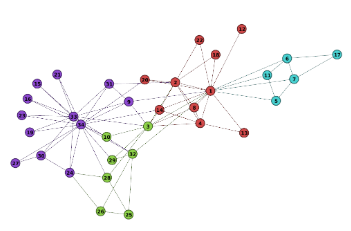
\includegraphics[width=2in]{images/karate_net.png}\Description{Karate Network}
% \caption{The karate network}
% \end{figure}

% \begin{figure*}
% 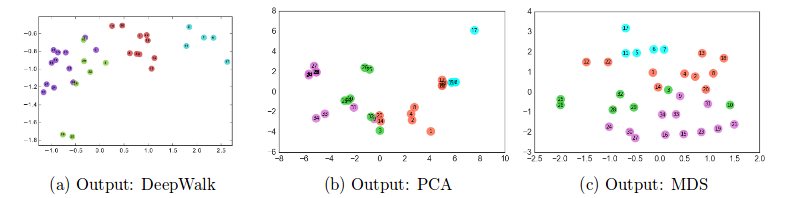
\includegraphics[width=7in]{images/karate_net_deepwalk.png}\Description{Karate Network Deepwalk}
% \caption{Shows the results of classification using DeepWalk vs traditional methods on the karate network}
% \end{figure*}

\subsection{Influence Network Learning}
Influence learning on a higher level can be defined as the effects of one node in the network on others. Influence is an intrinsic part of most of the networks found in real-world. Specifically, social media is completely dependent on the interaction between various users of the network. Any kind of interaction, be it in modern media or real-life, create influence. Influence can also be synonymous with information flow.

Traditionally, the influence was being modeled with a specialized domain-specific concept. For example, \cite{matsubara2012rise} defines social influence by modeling complex differential equations from an existing social model. A few other research uses behavior propagation modeling based on Ekman's model of emotion. \cite{wang2017gang} uses Guilt-by-association models which look into the features of the nodes in immediate neighborhood of the node under consideration. \cite{kempe2003maximizing} uses information diffusion mechanism to study the flow of information from source to across the network and further uses cascading to maximize the flow.

Influence network learning requires more data than just the nodes and the edges of the network. To model influence, we need information about every interaction between the nodes, for example, contents of the interaction, type of interaction, time of interaction, the response time, average response time, etc.

Most network embedding methods use and learn the network structure. But, they don't work on modeling the influence or the information flow. \cite{qiu2018deepinf} comes closest to the topic of this paper, where they use deep neural networks to predict the classification.

\hrule
x
\hrule

\section{Preliminaries}
\label{section_prelim}
In this section, we introduce the terminologies and theorems that have been used in further sections.

\subsection{Agents, Goods, Allocations, and Utilities}
Agents are a set of actors who try to claim the ownership over a set of goods. Goods are the set of objects which are to be allocated among the agents. Let us denote the set of $\mathit{n}$ agents with $\mathcal{N}$ and $\mathcal{M}$ be the set of $\mathit{m}$ indivisible goods.

Each agent have an associated utility for a particular good. In other words, each agent values a set of goods over others by a quantity. This is called a valuation function or an utility function. For agent $i$, the utility function is $f_i: M\mapsto \mathbb{R_+}$, where $\mathbb{R_+}$ is the set of positive real numbers. Here we assume each agent values the goods positively. We will encounter utility functions again in this section when we discuss some specific types of market later in the section.

An allocation is a distribution of goods into shares or portions. When we have only one quantity of each goods, each agent shows binary allocations. It owns/gets the good or it doesn't. It is illustrated in figure xyz1. If we have more than one count for any goods, an agent can get any permutation of it. We are assuming a single amount of each good unless specified otherwise. An allocation $\mathcal{A}_i\subseteq \mathcal{M}$ for any agent $i$.

For agent $i$, with an allocation $\mathcal{A}_i$ and its utility function for goods $f_i$, we can calculate the agent's total value of the allocation as
\begin{gather}
    F_i = \sum_{a \in \mathcal{A}_i} f_i(a)
\end{gather}

As mentioned previously, we will later see how this changes for different value functions.

% \begin{figure*}
% 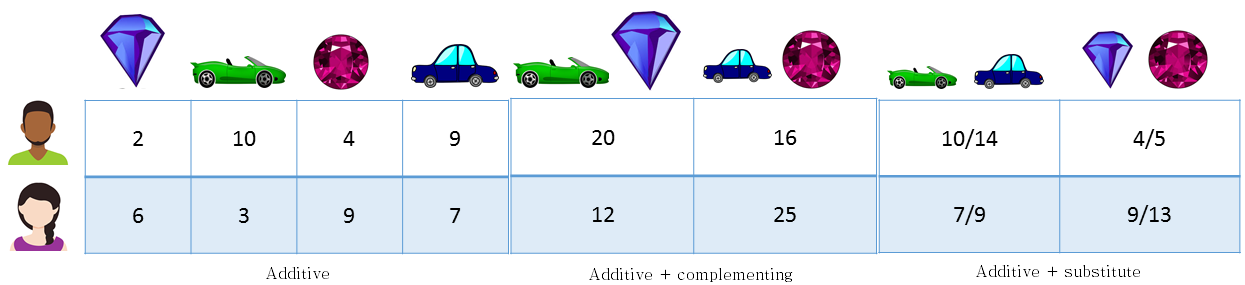
\includegraphics[width=7in]{images/utilities.png}\Description{Additive, complementary and substitute utilities}
% \caption{Additive, complementing, and substitute values in Inheritance distribution}
% \end{figure*}

\subsection{Additive goods and utilities}
Formally, additive goods/utilities are the ones who showcase mathematical additive properties. Additive goods are the ones whose utility is independent of others. Additive utilities are same as the one specified in previous section; that is, for agent $i$, the additive utility function is $u_i: M\mapsto \mathbb{R_+}$. Total utility of a set of goods/allocations is equal to the sum of all disjoint subsets.
\begin{gather}
    U_i = \sum_{a \in \mathcal{A}_i} u_{i,a}
\end{gather}

Where $\mathcal{A}_i$ is the allocation of goods to agent i and $u_{i,a}$ is agent i's utility for good a.

\subsection{Complementary goods and utilities}
\label{section_complementary}

Two goods are said to be complements if demand for one has some form of dependency over the demand of other. In other words, their demands are linked in such a way that increase in one raises the demand of the other, and same the decrease. A popular real-world example of complementary goods is razors blades. If the sell of razors increases, the demand for blades will rise too. This is an example of perfect complements. One can't use razors without blades or the other way. Real-world is full of such examples; burger and fries, hot dogs and buns, cars and gas, etc. Some of them are perfect complements, others are not.

In this paper, we define complements over pairs of adjacent goods. We denote complementing utilities for each agent i as: 

\begin{gather}
    v_i: \forall_{j < |M|/2} (M_{2j}, M_{2j+1})\mapsto \mathbb{R_+}
\end{gather}

An agent will earn the complementing utility if its allocation contains both the goods representing that value, otherwise not. If it does, it will be added to the additive utility to get the total utility of the allocation of agent i.

**How to write total utility in mathematical form?**

\begin{figure}
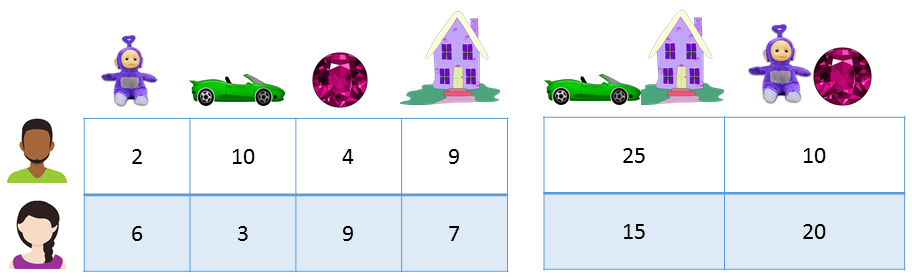
\includegraphics[width=3in]{images/complementary_values.png}\Description{Additive and complementing values in Inheritance distribution}
\caption{Additive and complementing utilities in inheritance allocation}
\end{figure}


\subsection{Substitute goods and utilities}
\label{section_substitute}

/* Filler. Replace this

Submodular, supermodular, subadditivity, superadditivity

Two goods are said to be substitutes if demand for one has some form of dependency over the demand of other. In other words, their demands are linked in such a way that increase in one raises the demand of the other, and same the decrease. A popular real-world example of complementary goods is razors blades. If the sell of razors increases, the demand for blades will rise too. This is an example of perfect complements. One can't use razors without blades or the other way. Real-world is full of such examples; burger and fries, hot dogs and buns, cars and gas, etc. Some of them are perfect complements, others are not.

In this paper, we define complements over pairs of adjacent goods. We denote complementing utilities for each agent i as: 

\begin{gather}
    v_i: \forall_{j < |M|/2} (M_{2j}, M_{2j+1})\mapsto \mathbb{R_+}
\end{gather}

An agent will earn the complementing utility if its allocation contains both the goods representing that value, otherwise not. If it does, it will be added to the additive utility to get the total utility of the allocation of agent i.

\begin{figure}
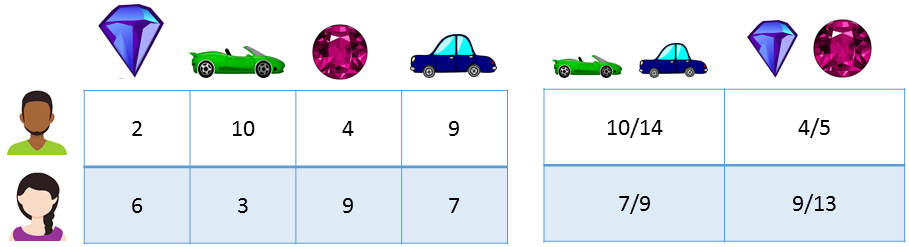
\includegraphics[width=3in]{images/substitute_values.png}\Description{Additive and substituting values in Inheritance distribution}
\caption{Additive and substitute utilities in inheritance allocation}
\end{figure}

*/

\subsection{Fairness, Envy, and Envy-freeness}
\label{section_envy}
Fairness is one of the primary criteria in any resource allocation problem. The notion of fairness differs with the definition of the allocation problem. Consider the problem of division of a cake among $n$ people. Each person should receive $n$th part of the cake. We extend the problem by starting with $m$ cakes. Share of each person should now be $m/n$. The fairness criterion here is very loose as the only constraint we are trying to satisfy is equal distribution among all. In the same problem, we introduce the concept of age of a person. A person should receive a portion of a cake with respect to the age. Young ones will get more cake than the older. The fairness criteria now is to strictly get more cake if younger and not necessarily equal if same age. The criteria can further be varied if we introduce other types of food and preferences of people over these types.

One fairness criterion studied extensively in literature is Envy-freeness. Envy is defined as an amount with which an agent prefers an allocation of someone else. 

\subsubsection{Definition 3.1} Envy.
An agent $i$ with a value of $v_{ia}$ for a good $a$ which is allocated to agent $j$ who has a value of $v_{ja}$ for the same good $a$ envies agent $j$ by an
amount $e_{ij} = v_{ja} - v_{ia}$. The entity $e_{ij} \geq 0$ implies agent $i$ does not envy agent $j$, whereas $|e_{ij}|$ is the amount of envy $i$ has for $j$ otherwise. Extending the same to the entire allocation $\mathcal{A}_i$ instead of a single good, $E_{ij} = V_i(\mathcal{A}_j) - V_i(\mathcal{A}_i)$, where $V_i$ is the value function for agent $i$, and $\mathcal{A}_i$ and $\mathcal{A}_j$ are allocations of $i$ and $j$, respectively.

Envy-freeness (EF) is a notion of fair allocation where every agent prefers their own allocation over that of any other agent. In other words, every agent feels their allocation is better than or at least as valuable as the allocation of any other agent.

\subsubsection{Definition 3.2} Envy-freeness (EF).
An allocation is envy-free if $\mathcal{A}_i \succeq_i \mathcal{A}_j \forall i,j$ where $\mathcal{A}_i$ and $\mathcal{A}_j$ is the allocation of $i$ and $j$, respectively. Given a value function $V_i$ for agent $i$, $V_i(\mathcal{A}_i) \geq V_i(\mathcal{A}_j)$ $\forall i,j$. 

For a simple cake division problem, each person would want a piece of size greater than or at least equal to any other person. No one would want to exchange their piece with anyone else. This results in everyone having same sized pieces of the cake.

In the extended version of the problem, the idea of envy should reflect the age of the person. In an envy-free allocation, each person will have a piece of cake according to their own age and ensuring the fact that they don't want the piece of any other person. 

Fair distribution of a cake is an example of divisible goods. There always exist an envy-free solution for the allocation of divisible goods [cite]. Though, increasing the number of agents, increases the complexity of the envy-free allocation and it may take a very long time for computation [cite].

The problem gets difficult for indivisible goods. In a simple example with one item and two agents, where both have positive utilities for the item, the item can only be allocated to one of the agents. No matter which agent gets the item, the other agent will always envy for not getting the item. Envy-free division can not be guaranteed in general for the case of indivisible goods. The problem of determining whether an allocation exists, which is envy-free, is computationally hard [cite].

For feasibility, we weaken the constraint on envy-freeness and attempt allocation under these constraint.

\begin{definition}{Envy-free up to one good (EF1) \cite{caragiannis2016unreasonable}}
\label{def_ef1}
An allocation $\mathcal{A}$ is envy-free up to one good (EF1) if for all agents $i$, $j$, agent $i$ will stop envying agent $j$ if a good $g$, for some $g$ in $\mathcal{A}_j$ is dropped from the allocations of agent $j$, $\mathcal{A}_j$. Formally,
$$
    \forall i,j \in \mathcal{N}, \exists g \in \mathcal{A}_j, V_i(\mathcal{A}_i) \geq V_i(\mathcal{A}_j \backslash \{g\})
$$
\end{definition}

We further relax the envy-freeness fairness criterion for up to $k$ goods.

\begin{definition}{Envy-free up to $k$ goods (EFk).}
\label{def_efk}
An allocation $\mathcal{A}$ is envy-free up to $k$ goods (EFk) if for all agents $i$, $j$, agent $i$ will stop envying agent $j$ if a set of goods $\mathcal{G} \subseteq \mathcal{A}_j$, such that $|\mathcal{G}| = k$, is dropped from the allocations of agent $j$, $\mathcal{A}_j$. Formally,
$$
    \forall i,j \in \mathcal{N}, k \leq |\mathcal{M}|, \exists \mathcal{G} \subseteq \mathcal{A}_j, |G| = k, V_i(\mathcal{A}_i) \geq V_i(\mathcal{A}_j \backslash \{\mathcal{G}\})
$$
\end{definition}

In other words, if agent $i$ doesn't envy agent $j$ once we drop some $k$ goods from agent $j$'s allocation $\mathcal{A}_j$, then the allocation is called envy-free up to $k$ goods (EFk).

Also, the definition \ref{def_efk} allows an EFk allocation to be EF(k+1), EF(k+2), and so on, as once we have an EFk allocation $ \exists G \subseteq \mathcal{A}$, $ |G|=k \ni V_i(\mathcal{A}_i) - V_i(\mathcal{A}_j \backslash G) \geq 0 $ and dropping more goods from agent $j$'s allocation would only increase $V_i(\mathcal{A}_i) - V_i(\mathcal{A}_j \backslash G)$ and not create any new envy.


\subsection{Welfare and Maximum Nash Welfare}
\label{section_welfare}
Welfare is a concept of an economic system which ensures happiness and well-being of all the participating agents with some agreed definition of happiness or well-being. It follows the idea of fairness from the previous section. A system which is fair to all the constituting members can be said to ensure the welfare of all the participants, and further, the welfare of the entire system. We adopt the terminology of welfare in the resource allocation problem. Given an allocation of goods among agents, we believe we have achieved welfare if we have a fair allocation for each agent.

Like fairness, the notion of welfare differs with the definition of the resource allocation problem. Following the example from the previous section, for the simple cake division problem, equal division of cake among all agents would achieve the welfare in cake distribution. In the extended version of the cake division problem, if each agent receives a fair amount of cake based on the fairness criterion of age, the division will ensure welfare of the system.

Three popular notions of welfare are often discussed in economics: utilitarian, egalitarian and Nash.

An utilitarian welfare strives to achieve maximum overall utility. In resource allocation problem, a good will be allocated to that agent who has the maximum value for it. This ensures the maximum possible usage of the goods. Here, the idea of fairness is specified as maximum utilization of the goods. In that sense, it provides the most efficient allocation. Utilitarian distribution does not ensure that each agent needs to receive some good. An agent who does not have the best value for any good, may not get any good. Also, it is possible that one may have best value for all of the goods and may end up receiving all the goods. In other words, utilitarian welfare, in trying to achieve the highest possible utility, does not ensure positive utility for all the participants.

An egalitarian welfare tries to maximize well-being or happiness of all agents. It strives to achieve equality of some type among all agents. In resource allocation problem, an egalitarian welfare system would not regard the utilities that agents have for various goods. A good should be allocated to an agent who owns the least amount. With a notion of equality defined, an egalitarian welfare provides the most fair allocation.

The simple cake division problem described above is both utilitarian and egalitarian. Every agent gets an equal share of the cake, and since every agent have the same value for the cake, the distribution achieves maximum efficiency. For the extended version of the cake division problem, the value for the cake is inversely proportional to the age of the person. The egalitarian welfare solution would allocate an equal amount of cake to everyone, whereas the utilitarian welfare solution would distribute cake based on the value.

The maximum Nash welfare (MNW) solution provides both fairness and efficiency. We follow the definition the MNW solution by Caragiannis, Ioannis, et al. \cite{caragiannis2016unreasonable}

\begin{definition}{Nash welfare (NW) or Nash product} \label{def_nw}
Nash welfare or Nash product is a product of utilities of agents for allocated goods with a condition that every agent values it's allocation positively

\begin{equation}
    NW(\mathcal{A}) = 
    \begin{cases}
    \prod_{i \in \mathcal{N}} V_i(\mathcal{A}_i), & \text{if } \forall i \in \mathcal{N}, V_i(\mathcal{A}_i) > 0 \\
    \text{not defined}, & \text{otherwise}
    \end{cases}
\end{equation}

for all agents $i$ in $\mathcal{N}$, where $V$ is the value function and $\mathcal{A}$ is the allocation.
\end{definition}

\begin{definition}{Maximum Nash welfare (MNW).} \label{def_mnw}
MNW allocation is the one that maximizes the Nash welfare among all possible allocations

$$
    \mathcal{A}^{MNW} = \operatorname{arg\,max}_{A \in \prod_{|\mathcal{N}|}(\mathcal{M})} NW(\mathcal{A})
$$
\end{definition}


Maximum Nash welfare is widely known for its welfare guarantees. MNW is found to satisfy interesting properties in a fair allocation problem. MNW is efficient with satisfaction of the Pareto optimality, and it has an attractive fairness property in the form of envy-freeness.

Pareto optimal (PO) allocation is the one in which it is not possible to make allocations of one agent better without making another agent's allocation worse. Pareto efficiency specifies the impossibility of improvement for one agent without affecting other agents negatively. PO is used as a property of efficient allocations because an allocation will not be Pareto if one can find an alternate allocation which improves the welfare for at least one agent without hurting the welfare of any other agent. With existence of no such improvement, PO represents the best possible scenario under such efficiency preference criteria.

\begin{definition}{Pareto optimality (PO).}
An allocation $\mathcal{A}$ is Pareto optimal if no other allocation $\mathcal{A'}$ is feasible such that $V_i(\mathcal{A}_i') \geq V_i(\mathcal{A}_i)$ for all agents $i \in \mathcal{N}$ with $ V_j(\mathcal{A}_j') > V_j(\mathcal{A}_j)$ for some agent $j \neq i$ where, $V_i$ is the value function for any agent $i \in \mathcal{N}$.
\end{definition}

\begin{theorem}
Every MNW allocation is Pareto optimal (PO) over indivisible goods.
\end{theorem}

\begin{proof}
We follow a simple proof of Pareto optimality for MNW by Caragiannis, Ioannis, et al. \cite{caragiannis2016unreasonable}. It is trivial for every MNW allocation $\mathcal{A}$ to be PO because any alternate allocation $\mathcal{A}'$ that increases the utility of one agent without decreasing the utility of any other agent would result in increase in the Nash welfare of the alternate allocation $\mathcal{A}'$, that is $NW(\mathcal{A}') > NW(\mathcal{A})$, contradicting the assumption that the original MNW allocation $\mathcal{A}$ had the maximum/optimal NW of all the possible allocations. 
\end{proof}

Maximum Nash welfare allocation satisfy the elusive fairness property of envy-freeness (EF) defined in the previous section. This is further studied and proved in the next section.

With PO and EF, the maximum Nash welfare, in a great degree of simplicity, is one of the rare algorithms providing us with both efficiency and fairness standards. It is a good balance between the utilitarian vs. egalitarian trade-off. Also, attempting to maximize for utilitarian or egalitarian welfare conditions results in non-EF allocations \cite{caragiannis2016unreasonable}. In that sense, MNW allocation prevails over utilitarian and egalitarian allocation criteria for the strong PO and EF guarantees that it ensures.

\section{Experiments}
\label{section_experiments}
In this section, we describe the data, computations, and analysis of the features of the data.

We simulate the problem with $n = 2$ agents competing for allocation of $m$ goods where $m \in \{10, 8, 6, 4\}$. The goods are unrelated, and independent. Each agent has some utility for each of the goods. We generate $m$ additive utilities for each agent at random over $[0, 100)$ representing agent's value for $m$ goods. We further generate $m/2$ complementary utilities for each agent at random over $[0, 100)$ representing agent's valuation for pairs of goods. Each complementary utility represents the collective value an agent would get if both the goods are allocated to the agent. We generate 100 samples each with random seed [10, 20) for reproducibility. Overall, we have $1000$ such examples for each value of $m \in {10, 8, 6, 4}$. In addition to that, we map these examples on to four types of goods showing : i) Additive utilities ii) Complementing utilities iii) Substituting utilities type 1 iv) Substituting utilities type 2.  MNW is computed for each of these sample with respect to four types of utilities with algorithm 1.

\BlankLine

% Maximum Nash Welfare computation - value function abstracted
\begin{algorithm}
\caption{ Computing an MNW allocation }
\SetAlgoLined
\KwIn{ Agents $\mathcal{N}$, resources $\mathcal{M}$, value function $value\_f$, additive utilities $AU$, complementary/substituting utilities $CSU$ }
\KwOut{ An MNW allocation $ \mathcal{A}^{MNW}$ }
 $Max\_NW \leftarrow 0 $ \;
 $\mathcal{A}_{Max\_NW} \leftarrow \phi $ \;
 \For{all possible allocations $ \mathcal{A} (N \times M) $}{
  $NW_\mathcal{A} \leftarrow \prod_{i \in \mathcal{N}} value\_f(\mathcal{A}_i, AU, CSU) $ \;
  \If{$NW_{\mathcal{A}} > Max\_NW $}{
   $Max\_NW \leftarrow NW_{\mathcal{A}}$ \;
   $\mathcal{A}_{Max\_NW} \leftarrow \mathcal{A} $ \;
  }
 }
\end{algorithm}

% Nash Welfare/Product computation
% For additive, complementing, substituting (type 1 and 2) utilities
\begin{algorithm}
\caption{ Computing NW }
\SetAlgoLined

Pairwise Allocation: \\
$ PA = (\mathcal{A}) \rightarrow [min(\mathcal{A}_{i,2j}, \mathcal{A}_{i,2j+1}) \forall i \in \mathcal{N}, j < |\mathcal{M}|/2] $

\BlankLine

Substituting utilities - type 1: \\
$ SU_1 = (AU) \rightarrow [max(AU_{i,2j}, AU_{i,2j+1}) \forall i \in \mathcal{N}, j < |\mathcal{M}|/2] $

\BlankLine

Substituting utilities - type 2: \\
$ SU_2 = (AU) \rightarrow [(AU_{i,2j} + AU_{i,2j+1}) - rand(0, min(AU_{i,2j}, AU_{i,2j+1}))) \forall i \in \mathcal{N}, j < |\mathcal{M}|/2] $

\BlankLine
\BlankLine

$ NW_{additive} = (\mathcal{A}, AU) \rightarrow \mathcal{A} \cdot AU $

$ NW_{compl} = (\mathcal{A}, AU, CU) \rightarrow \mathcal{A} \cdot AU + PA(\mathcal{A}) \cdot CU $

$ NW_{subst1} = (\mathcal{A}, AU) \rightarrow \mathcal{A} \cdot (AU - PA(\mathcal{A})) + PA(\mathcal{A}) \cdot SU_1(AU) $

$ NW_{subst2} = (\mathcal{A}, AU) \rightarrow \mathcal{A} \cdot (AU - PA(\mathcal{A})) + PA(\mathcal{A}) \cdot SU_2(AU) $

\end{algorithm}

% Discussion on analysis of experiements starts here

% Percent EFness
\begin{figure}[h!]
  \centering
  \begin{subfigure}[b]{0.3\linewidth}
    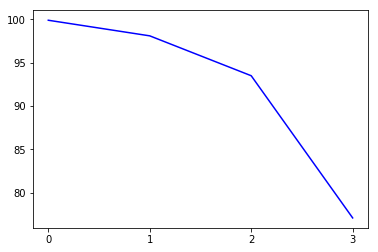
\includegraphics[width=\linewidth]{images/add/ef0_percent.png}
    \caption{}
  \end{subfigure}
  \begin{subfigure}[b]{0.3\linewidth}
    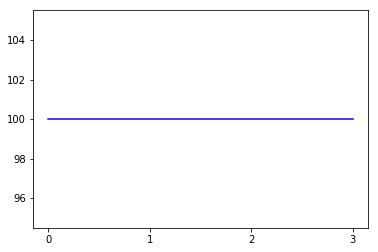
\includegraphics[width=\linewidth]{images/add/ef1_percent.png}
    \caption{}
  \end{subfigure}
  \begin{subfigure}[b]{0.3\linewidth}
    \includegraphics[width=\linewidth]{images/add/ef2_percent.png}
    \caption{}
  \end{subfigure}
  
  \begin{subfigure}[b]{0.3\linewidth}
    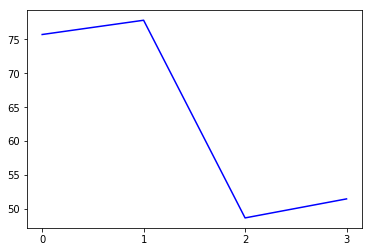
\includegraphics[width=\linewidth]{images/compl/ef0_percent.png}
    \caption{}
  \end{subfigure}
  \begin{subfigure}[b]{0.3\linewidth}
    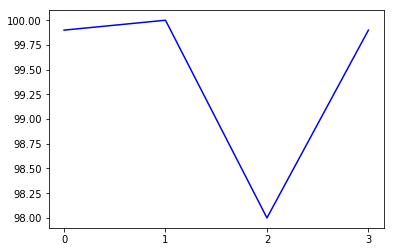
\includegraphics[width=\linewidth]{images/compl/ef1_percent.png}
    \caption{}
  \end{subfigure}
  \begin{subfigure}[b]{0.3\linewidth}
    \includegraphics[width=\linewidth]{images/compl/ef2_percent.png}
    \caption{}
  \end{subfigure}
    
  \begin{subfigure}[b]{0.3\linewidth}
    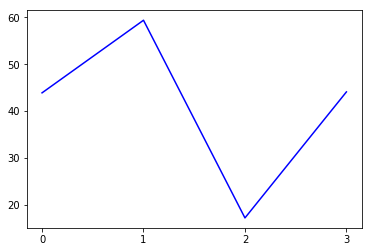
\includegraphics[width=\linewidth]{images/subst1/ef0_percent.png}
    \caption{}
  \end{subfigure}
  \begin{subfigure}[b]{0.3\linewidth}
    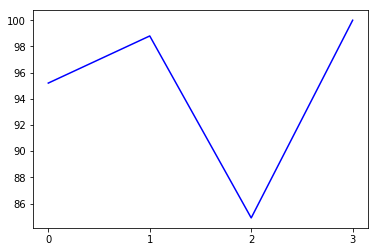
\includegraphics[width=\linewidth]{images/subst1/ef1_percent.png}
    \caption{}
  \end{subfigure}
  \begin{subfigure}[b]{0.3\linewidth}
    \includegraphics[width=\linewidth]{images/subst1/ef2_percent.png}
    \caption{}
  \end{subfigure}
    
  \begin{subfigure}[b]{0.3\linewidth}
    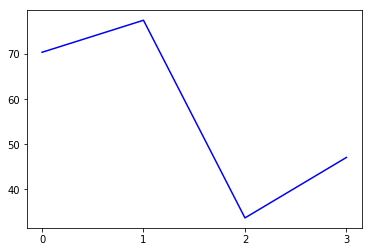
\includegraphics[width=\linewidth]{images/subst2/ef0_percent.png}
    \caption{}
  \end{subfigure}
  \begin{subfigure}[b]{0.3\linewidth}
    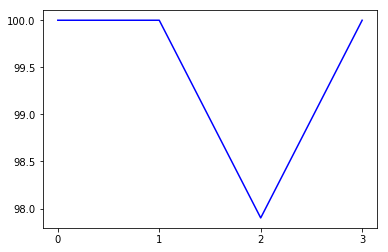
\includegraphics[width=\linewidth]{images/subst2/ef1_percent.png}
    \caption{}
  \end{subfigure}
  \begin{subfigure}[b]{0.3\linewidth}
    \includegraphics[width=\linewidth]{images/subst2/ef2_percent.png}
    \caption{}
  \end{subfigure}
  \caption{Percent EFk}
  \label{fig:efk}
  \small
    (a), (b), and (c) represent percent MNW allocations satisfying EF0, EF1, and EF2, respectively for additive utilities. (d), (e), (f), (g), (h), (i), (j), (k), and (l) represent that for complementing, substituting type-1, substituting type-2 utilities, respectively.
\end{figure}


Figure 4 shows the percent of samples which satisfies the envy-freeness specific criteria. Simple additive utilities gradually creates more envy with the decrease in number of goods as seen in Figure 4a. Figure 4a, 4b, and 4c collectively provides the experimental proof for envy-freeness up to one good (EF1) property of MNW allocations with additive valuations \cite{caragiannis2016unreasonable}. Figure 4f, 4i, and 4l, indicates pairwise complementary and substituting utilities follow envy-freeness up to 2 goods (EF2). Complementing and substituting utilities also showcase surprisingly high, if not perfect, EF1. In particular, substituting type-1 utilities for 4 goods and type-2 for 10, 8, and 4 goods have 100\% EF1.


% Mean Envy
\begin{figure}[h!]
  \centering
  \begin{subfigure}[b]{0.3\linewidth}
    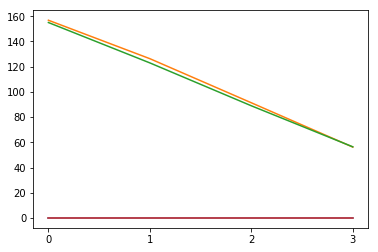
\includegraphics[width=\linewidth]{images/add/ef0_means.png}
    \caption{}
  \end{subfigure}
  \begin{subfigure}[b]{0.3\linewidth}
    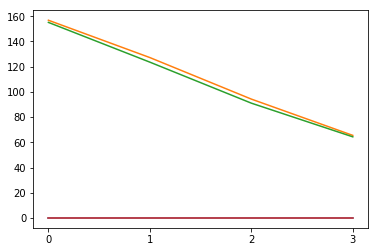
\includegraphics[width=\linewidth]{images/add/ef1_means.png}
    \caption{}
  \end{subfigure}
  \begin{subfigure}[b]{0.3\linewidth}
    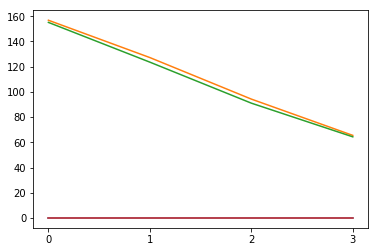
\includegraphics[width=\linewidth]{images/add/ef2_means.png}
    \caption{}
  \end{subfigure}
  
  \begin{subfigure}[b]{0.3\linewidth}
    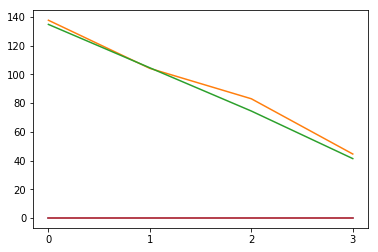
\includegraphics[width=\linewidth]{images/compl/ef0_means.png}
    \caption{}
  \end{subfigure}
  \begin{subfigure}[b]{0.3\linewidth}
    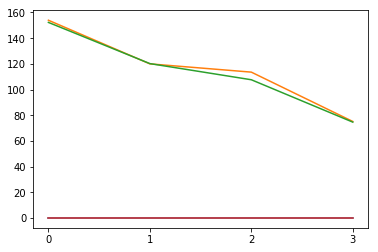
\includegraphics[width=\linewidth]{images/compl/ef1_means.png}
    \caption{}
  \end{subfigure}
  \begin{subfigure}[b]{0.3\linewidth}
    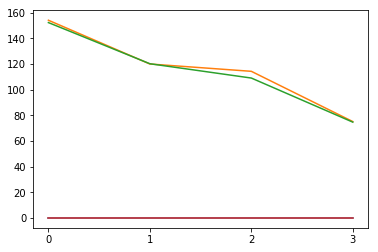
\includegraphics[width=\linewidth]{images/compl/ef2_means.png}
    \caption{}
  \end{subfigure}
    
  \begin{subfigure}[b]{0.3\linewidth}
    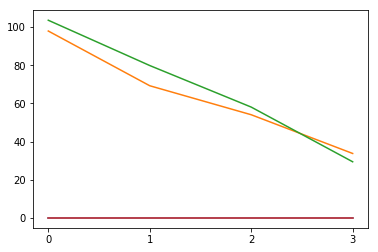
\includegraphics[width=\linewidth]{images/subst1/ef0_means.png}
    \caption{}
  \end{subfigure}
  \begin{subfigure}[b]{0.3\linewidth}
    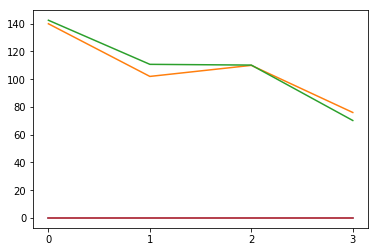
\includegraphics[width=\linewidth]{images/subst1/ef1_means.png}
    \caption{}
  \end{subfigure}
  \begin{subfigure}[b]{0.3\linewidth}
    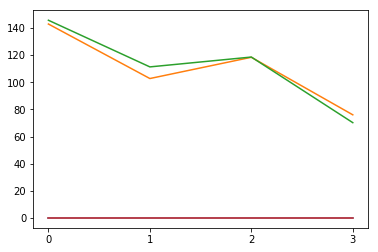
\includegraphics[width=\linewidth]{images/subst1/ef2_means.png}
    \caption{}
  \end{subfigure}
    
  \begin{subfigure}[b]{0.3\linewidth}
    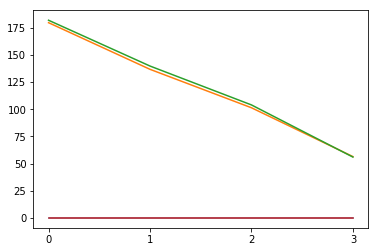
\includegraphics[width=\linewidth]{images/subst2/ef0_means.png}
    \caption{}
  \end{subfigure}
  \begin{subfigure}[b]{0.3\linewidth}
    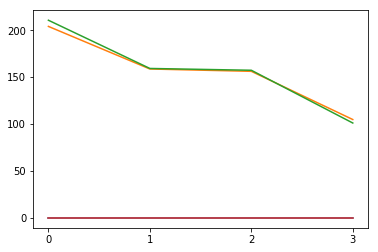
\includegraphics[width=\linewidth]{images/subst2/ef1_means.png}
    \caption{}
  \end{subfigure}
  \begin{subfigure}[b]{0.3\linewidth}
    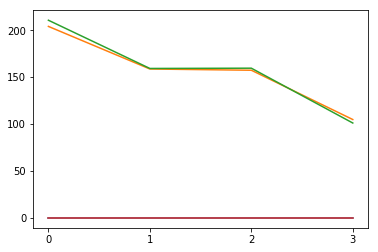
\includegraphics[width=\linewidth]{images/subst2/ef2_means.png}
    \caption{}
  \end{subfigure}
  \caption{Mean envy}
  \label{fig:efk}
  \small
    (a), (b), and (c) represent mean envy present in MNW allocations after dropping 0, 1, and 2 goods, respectively for additive utilities. (d), (e), (f), (g), (h), (i), (j), (k), and (l) represent that for complementing, substituting type-1, substituting type-2 utilities, respectively.
\end{figure}

% Mean Positive Envy
\begin{figure}[h!]
  \centering
  \begin{subfigure}[b]{0.3\linewidth}
    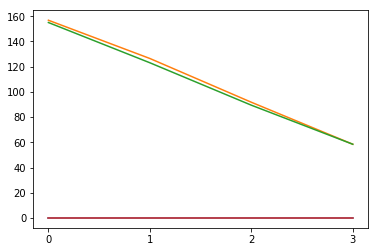
\includegraphics[width=\linewidth]{images/add/ef0_means_pos.png}
    \caption{}
  \end{subfigure}
  \begin{subfigure}[b]{0.3\linewidth}
    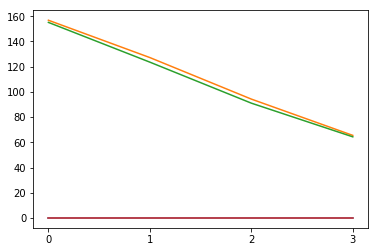
\includegraphics[width=\linewidth]{images/add/ef1_means_pos.png}
    \caption{}
  \end{subfigure}
  \begin{subfigure}[b]{0.3\linewidth}
    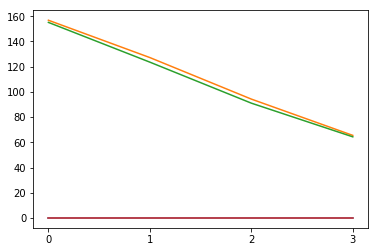
\includegraphics[width=\linewidth]{images/add/ef2_means_pos.png}
    \caption{}
  \end{subfigure}
  
  \begin{subfigure}[b]{0.3\linewidth}
    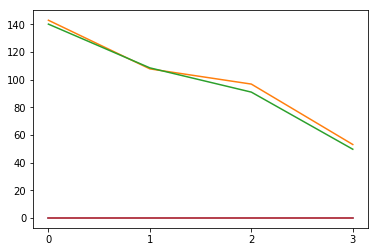
\includegraphics[width=\linewidth]{images/compl/ef0_means_pos.png}
    \caption{}
  \end{subfigure}
  \begin{subfigure}[b]{0.3\linewidth}
    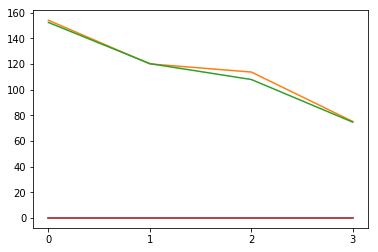
\includegraphics[width=\linewidth]{images/compl/ef1_means_pos.png}
    \caption{}
  \end{subfigure}
  \begin{subfigure}[b]{0.3\linewidth}
    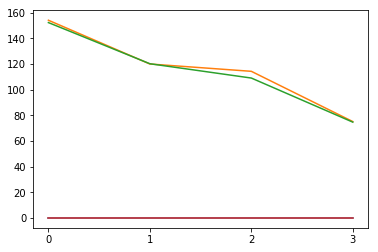
\includegraphics[width=\linewidth]{images/compl/ef2_means_pos.png}
    \caption{}
  \end{subfigure}
    
  \begin{subfigure}[b]{0.3\linewidth}
    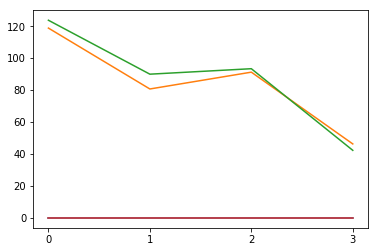
\includegraphics[width=\linewidth]{images/subst1/ef0_means_pos.png}
    \caption{}
  \end{subfigure}
  \begin{subfigure}[b]{0.3\linewidth}
    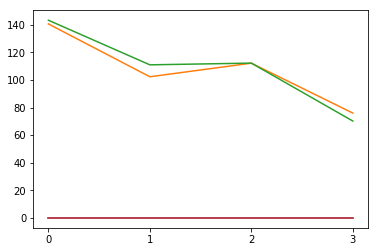
\includegraphics[width=\linewidth]{images/subst1/ef1_means_pos.png}
    \caption{}
  \end{subfigure}
  \begin{subfigure}[b]{0.3\linewidth}
    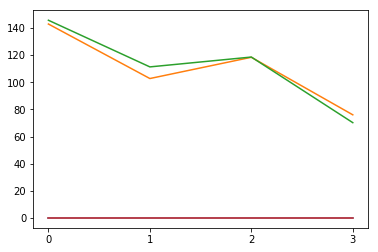
\includegraphics[width=\linewidth]{images/subst1/ef2_means_pos.png}
    \caption{}
  \end{subfigure}
    
  \begin{subfigure}[b]{0.3\linewidth}
    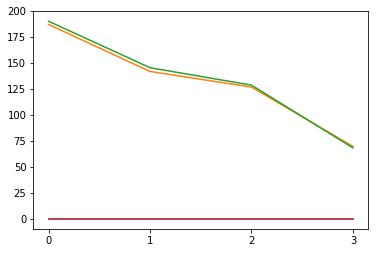
\includegraphics[width=\linewidth]{images/subst2/ef0_means_pos.png}
    \caption{}
  \end{subfigure}
  \begin{subfigure}[b]{0.3\linewidth}
    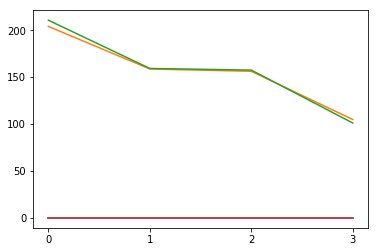
\includegraphics[width=\linewidth]{images/subst2/ef1_means_pos.png}
    \caption{}
  \end{subfigure}
  \begin{subfigure}[b]{0.3\linewidth}
    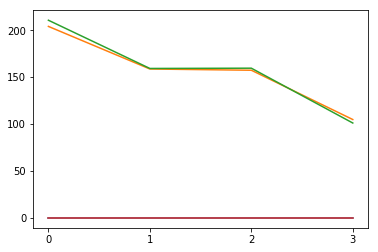
\includegraphics[width=\linewidth]{images/subst2/ef2_means_pos.png}
    \caption{}
  \end{subfigure}
  \caption{Mean positive envy}
  \label{fig:efk}
  \small
    (a), (b), and (c) represent mean positive envy (non-envy) present in MNW allocations after dropping 0, 1, and 2 goods, respectively for additive utilities. (d), (e), (f), (g), (h), (i), (j), (k), and (l) represent that for complementing, substituting type-1, substituting type-2 utilities, respectively.
\end{figure}

% Mean Negative Envy
\begin{figure}[h!]
  \centering
  \begin{subfigure}[b]{0.3\linewidth}
    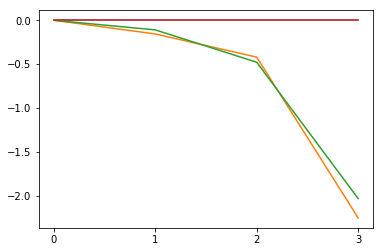
\includegraphics[width=\linewidth]{images/add/ef0_means_neg.png}
    \caption{}
  \end{subfigure}
  \begin{subfigure}[b]{0.3\linewidth}
    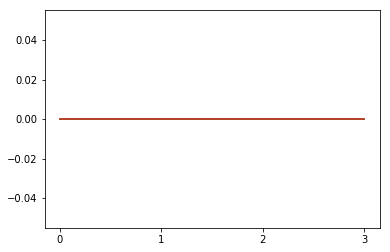
\includegraphics[width=\linewidth]{images/add/ef1_means_neg.png}
    \caption{}
  \end{subfigure}
  \begin{subfigure}[b]{0.3\linewidth}
    \includegraphics[width=\linewidth]{images/add/ef2_means_neg.png}
    \caption{}
  \end{subfigure}
  
  \begin{subfigure}[b]{0.3\linewidth}
    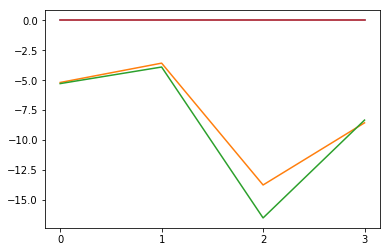
\includegraphics[width=\linewidth]{images/compl/ef0_means_neg.png}
    \caption{}
  \end{subfigure}
  \begin{subfigure}[b]{0.3\linewidth}
    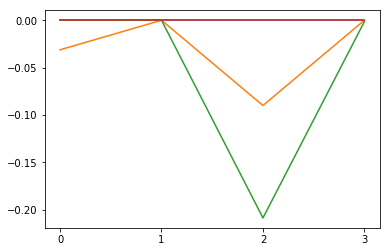
\includegraphics[width=\linewidth]{images/compl/ef1_means_neg.png}
    \caption{}
  \end{subfigure}
  \begin{subfigure}[b]{0.3\linewidth}
    \includegraphics[width=\linewidth]{images/compl/ef2_means_neg.png}
    \caption{}
  \end{subfigure}
    
  \begin{subfigure}[b]{0.3\linewidth}
    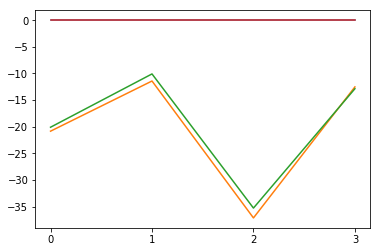
\includegraphics[width=\linewidth]{images/subst1/ef0_means_neg.png}
    \caption{}
  \end{subfigure}
  \begin{subfigure}[b]{0.3\linewidth}
    \includegraphics[width=\linewidth]{images/subst1/ef1_means_neg.png}
    \caption{}
  \end{subfigure}
  \begin{subfigure}[b]{0.3\linewidth}
    \includegraphics[width=\linewidth]{images/subst1/ef2_means_neg.png}
    \caption{}
  \end{subfigure}
    
  \begin{subfigure}[b]{0.3\linewidth}
    \includegraphics[width=\linewidth]{images/subst2/ef0_means_neg.png}
    \caption{}
  \end{subfigure}
  \begin{subfigure}[b]{0.3\linewidth}
    \includegraphics[width=\linewidth]{images/subst2/ef1_means_neg.png}
    \caption{}
  \end{subfigure}
  \begin{subfigure}[b]{0.3\linewidth}
    \includegraphics[width=\linewidth]{images/subst2/ef2_means_neg.png}
    \caption{}
  \end{subfigure}
  \caption{Mean Negative envy}
  \label{fig:efk}
  \small
    (a), (b), and (c) represent mean negative envy (envy) present in MNW allocations after dropping 0, 1, and 2 goods, respectively for additive utilities. (d), (e), (f), (g), (h), (i), (j), (k), and (l) represent that for complementing, substituting type-1, substituting type-2 utilities, respectively.
\end{figure}


Figure 5 plots mean envy between the agents after dropping 0, 1, and 2 goods for all MNW allocations. Mean envy-freeness raises with drops of 0, 1 and 2 goods as expected. The difference is greater from EF0 to EF1 than from EF1 to EF2 which is almost the same. This indicates when agents drop the first good in EF1 calculation, though it is known to drop the one which is valued the most by others, the first drop has a very high utility. Also noticeable is the decrease in envy-freeness with decrease in the number of goods. It is visible regardless of the type of utility or the number of goods being dropped. Figure 6 shows the mean positive envy (non-envy) in the allocation which closely follows and reflects the figure 5 mean envy plot.

Figure 7 plots the mean negative envy in the allocations after dropping 0, 1, and 2 goods for EF0, EF1, and EF2, respectively. Mean negative envy plot reflects association with Figure 4 - Percent EFk. It is the plot of envy values for the agents who negatively envies other agents. Similar to Figure 4, EF2 shows zero envy. The same high EF1 pattern as Figure 4 is visible in Figure 7 with some allocations showing zero negative envy.


% % DFs additive
% \begin{figure}[h!]
%   \centering
%   \begin{subfigure}[b]{0.47\linewidth}
%     \includegraphics[width=\linewidth]{images/add/pdf_additive_10.png}
%     \caption{}
%   \end{subfigure}
%   \begin{subfigure}[b]{0.47\linewidth}
%     \includegraphics[width=\linewidth]{images/add/pdf_additive_8.png}
%     \caption{}
%   \end{subfigure}
%   \begin{subfigure}[b]{0.47\linewidth}
%     \includegraphics[width=\linewidth]{images/add/pdf_additive_6.png}
%     \caption{}
%   \end{subfigure}
%   \begin{subfigure}[b]{0.47\linewidth}
%     \includegraphics[width=\linewidth]{images/add/pdf_additive_4.png}
%     \caption{}
%   \end{subfigure}
%   \caption{Envy distribution curve for Additive Utilities}
%   \label{fig:efk}
%   \small
%     Envy distribution of the entire sample space with additive utilities after dropping 0, 1, and 2 goods for number of goods (a) $m = 10$, (b) $m = 8$, (c) $m = 6$, (d) $m = 4$
% \end{figure}

% % DFs complementing
% \begin{figure}[h!]
%   \centering
%   \begin{subfigure}[b]{0.47\linewidth}
%     \includegraphics[width=\linewidth]{images/compl/pdf_complementing_10.png}
%     \caption{}
%   \end{subfigure}
%   \begin{subfigure}[b]{0.47\linewidth}
%     \includegraphics[width=\linewidth]{images/compl/pdf_complementing_8.png}
%     \caption{}
%   \end{subfigure}
%   \begin{subfigure}[b]{0.47\linewidth}
%     \includegraphics[width=\linewidth]{images/compl/pdf_complementing_6.png}
%     \caption{}
%   \end{subfigure}
%   \begin{subfigure}[b]{0.47\linewidth}
%     \includegraphics[width=\linewidth]{images/compl/pdf_complementing_4.png}
%     \caption{}
%   \end{subfigure}
%   \caption{Envy distribution curve for Complementing Utilities}
%   \label{fig:efk}
%   \small
%     Envy distribution of the entire sample space with complementing utilities after dropping 0, 1, and 2 goods for number of goods (a) $m = 10$, (b) $m = 8$, (c) $m = 6$, (d) $m = 4$
% \end{figure}

% % DFs substituting type-1
% \begin{figure}[h!]
%   \centering
%   \begin{subfigure}[b]{0.47\linewidth}
%     \includegraphics[width=\linewidth]{images/subst1/pdf_subst1_10.png}
%     \caption{}
%   \end{subfigure}
%   \begin{subfigure}[b]{0.47\linewidth}
%     \includegraphics[width=\linewidth]{images/subst1/pdf_subst1_8.png}
%     \caption{}
%   \end{subfigure}
%   \begin{subfigure}[b]{0.47\linewidth}
%     \includegraphics[width=\linewidth]{images/subst1/pdf_subst1_6.png}
%     \caption{}
%   \end{subfigure}
%   \begin{subfigure}[b]{0.47\linewidth}
%     \includegraphics[width=\linewidth]{images/subst1/pdf_subst1_4.png}
%     \caption{}
%   \end{subfigure}
%   \caption{Envy distribution curve for Substituting type 1 Utilities}
%   \label{fig:efk}
%   \small
%     Envy distribution of the entire sample space with substituting utilities type 1 after dropping 0, 1, and 2 goods for number of goods (a) $m = 10$, (b) $m = 8$, (c) $m = 6$, (d) $m = 4$
% \end{figure}

% % DFs substituting type-2
% \begin{figure}[h!]
%   \centering
%   \begin{subfigure}[b]{0.47\linewidth}
%     \includegraphics[width=\linewidth]{images/subst2/pdf_subst2_10.png}
%     \caption{}
%   \end{subfigure}
%   \begin{subfigure}[b]{0.47\linewidth}
%     \includegraphics[width=\linewidth]{images/subst2/pdf_subst2_8.png}
%     \caption{}
%   \end{subfigure}
%   \begin{subfigure}[b]{0.47\linewidth}
%     \includegraphics[width=\linewidth]{images/subst2/pdf_subst2_6.png}
%     \caption{}
%   \end{subfigure}
%   \begin{subfigure}[b]{0.47\linewidth}
%     \includegraphics[width=\linewidth]{images/subst2/pdf_subst2_4.png}
%     \caption{}
%   \end{subfigure}
%   \caption{Envy distribution curve for Substituting type 2 Utilities}
%   \label{fig:efk}
%   \small
%     Envy distribution of the entire sample space with substituting utilities type 2 after dropping 0, 1, and 2 goods for number of goods (a) $m = 10$, (b) $m = 8$, (c) $m = 6$, (d) $m = 4$
% \end{figure}


Figure 8-11 plot the distributions of envy for simulated 1000 samples. As discussed about other plots, the decrease in number of goods can directly be seen in increase in number of envied allocations. These curves give a nice shape to the envy calculations before and after dropping goods for EF0, EF1, and EF2 calculations. Figure 8-11 show both, final envy after dropping the good and that sorted on the sampling x-axis which forms a smooth shape with rest of the distribution curve.

\section{MNW and EFk}
\label{section_proof}
In this section, we analyze the relation between maximum Nash welfare and envy-freeness up to k goods.

We already know MNW allocations for additive utility values are envy-free up to one good (EF1) \cite{caragiannis2016unreasonable}. The experiments on goods with additive utilities in previous section provide the experimental evidence to that fact.

In previous section, we conduct experiments on complementary and substitute goods. We have simulated the complements and substitutes of the goods in the market in terms of the dependency of utility valuation for pairs of goods. An interesting fact emerge from the plots is that, all of the MNW allocations are envy-freeness up to 2 goods.

We classify complementary and substitute valuations as bonded goods.

\begin{definition}{Additively bonded goods valuation.}
Bonded good is the good $x \in \mathcal{M}$ whose value $V_i(x), \forall i \in \mathcal{N}$ varies with whether the agent gets some other set of goods $Y \subseteq \mathcal{M}$ in allocation $\mathcal{A}$ or not and the value is additive.
\end{definition}

To elaborate further, suppose each agent have a value for each of the goods. If we can get a total utility for an agent by adding his values mapped to the goods that the agent owns, we have additively bonded goods with dependency of up to 1 good (all goods depend on themselves and no one else). Now we introduce utility function which is computed based on the fact that an agent owns a pair of goods. In this case, if an agent owns a pair, the value will be different that if the agent owns any one of the goods from the pair. But the total utility for the allocation can still be computed by adding the value for the pair instead of the individual goods. We call this additively bonded goods with dependency of up to 2 goods. On the same lines, if we have a value defined for getting a set of $k$ goods and the total utility can still be computed by adding the value of $k$ goods instead of any of the subsets, that can be called as additively bonded goods with dependency of up to $k$ goods.

The total utility of additively bonded goods with dependency of up to $k$ goods will be equal to the addition of values of subsets of the allocation.

\begin{equation}
\label{eq_abgv}
\begin{gathered}
    V_i(\mathcal{A}_i) = \operatorname{maximize} \sum_{j=0}^{k-1} V^{k-j}_i(\mathcal{A}^{k-j}_i) \\
    V_i(\mathcal{A}_i) = \operatorname{maximize} V^k_i(\mathcal{A}^k_i) + V^{k-1}_i(\mathcal{A}^{k-1}_i) + ... + V^1_i(\mathcal{A}^{1}_i)
\end{gathered}
\end{equation}

where $V$ is the valuation of allocation $\mathcal{A}$ for agent $i$. 

Extending the idea of EF1 of additive goods \cite{caragiannis2016unreasonable}, in this section, we formally affirm the envy-freeness up to $k$ goods (EFk) for additively bonded goods with dependency of up to $k$ goods.

\begin{theorem}
Every MNW allocation is envy free up to $k$ goods (EFk), for additively bonded valuations over indivisible goods where the valuations of an agent for goods show additive dependency on $k$ other goods.
\end{theorem}

\begin{proof}
By definition \ref{def_efk}, for all agent's $i, j \in \mathcal{N}$, an EFk allocation contains an agent $i$ who envies some agent $j$ even after dropping $k-1$ goods from agent $j$'s allocation and stops envying after dropping $k$th good. Also, if an allocation is EFk, then definition \ref{def_efk} permits the allocation to be EF(k+$i$) for $0 \leq i \leq |\mathcal{M}|$. So the only assertion to prove is guaranteed existence of EFk.

We approach this proof by contradiction. We start with a MNW allocation $\mathcal{A}$ being not EFk, so that agent $i$ envies agent $j$ even after removing $k$ goods from agent $j$'s allocation $\mathcal{A}_j$.

Let $G^* = \operatorname{arg\,min}_{G \subseteq \mathcal{A}_j, |G| \leq k, V_i(G)>0} V_j(G)/V_i(G)$. $G^*$ is a set of goods such that $|G| \leq k$. $G^*$ is well-defined because agent $i$ envying agent $j$ implies that agent $i$ has a positive envy for a set of at most $k$ goods in the allocation of agent $j$, $\mathcal{A}_j$. 

Let $\mathcal{A}'$ denote the allocation obtained from moving $G^*$ from agent $j$ to agent $i$ in $\mathcal{A}$. With this movement, we need to show $NW(\mathcal{A}') > NW(\mathcal{A})$, which will contradict the optimality of MNW assumption of $\mathcal{A}$ we began with.
$$
    NW(\mathcal{A}') > NW(\mathcal{A})
$$
$$
    \frac{NW(\mathcal{A}')}{NW(\mathcal{A})} > 1
$$
The ratio is valid, as we define $NW(\mathcal{A}) > 0$ always valid in definition \ref{def_nw}.

For all other agents $p$ not a part of the exchange, the value of allocation $\mathcal{A}_p$ does not change. That is, $\forall p \in \mathcal{N}\backslash\{i,j\}, V_p(\mathcal{A}'_p) = V_p(\mathcal{A}_p)$

Since MNW is Pareto optimal (PO) and goods are additively bonded, we can write,
$$
    V_i(\mathcal{A}'_i) = V_i(\mathcal{A}_i) + V_i(G^*)
$$
$$
    V_j(\mathcal{A}'_j) = V_j(\mathcal{A}_j) - V_j(G^*)
$$
Here, $V(G^*)$ represents maximum value derived by agents $i$ and $j$ from $G^*$ for $|G| \leq k$

So, backing up to the ratio of Nash welfare of the original and the modified allocations,

\begin{equation}
\label{eq_prooffinal}
\begin{gathered}
    \frac{NW(\mathcal{A}')}{NW(\mathcal{A})} > 1 \Leftrightarrow \left[\frac{V_i(\mathcal{A}_i) + V_i(G^*)}{V_j(\mathcal{A}_j) - V_j(G^*)}\right] \\
    \Leftrightarrow \left[1 - \frac{V_j(G^*)}{V_j(\mathcal{A}_j)}\right] \cdot \left[1 + \frac{V_i(G^*)}{V_i(\mathcal{A}_i)}\right] \\
    \Leftrightarrow \frac{V_j(G^*)}{V_i(G^*)} \cdot \left[V_i(\mathcal{A}_i) + V_i(G^*) \right] < V_j(\mathcal{A}_j)
\end{gathered}
\end{equation}

using the simple algebraic property for ratio, choice of $G^*$ and equation \ref{eq_abgv}
\begin{equation}
\label{eq_proofmul1}
    \frac{V_j(G^*)}{V_i(G^*)} \leq \frac{\sum_{G \in \mathcal{A}_j}V_j(G)}{\sum_{G \in \mathcal{A}_j}V_i(G)} = \frac{V_j(\mathcal{A}_j)}{V_i(\mathcal{A}_j)}
\end{equation}

Since agent $i$ envies $j$ even after removing $g^*$ from agent $j$'s allocations, we can write,
\begin{equation}
\label{eq_proofmul2}
\begin{gathered}
    V_i(\mathcal{A}_i) < v_i(\mathcal{A}_j) - V_i(G^*) \\
    V_i(\mathcal{A}_i) + V_i(G^*) < v_i(\mathcal{A}_j)
\end{gathered}
\end{equation}

Multiplying equations \ref{eq_proofmul1} and \ref{eq_proofmul2}, gives us equation \ref{eq_prooffinal} required to prove the theorem.

Since $G^* \subseteq \mathcal{A}_j where |G| \leq k$ and maximum possibility of $k$ in equation \ref{eq_abgv} used to arrive at equation \ref{eq_proofmul1}, we prove the theorem that the allocations are EFk.

\end{proof}

\section{Conclusion and Future Work}
\label{section_conclusion}

The primary aim of this paper is to analyze and prove the envy-freeness bounds for specialized markets that showcase different utilities than the generic additive utilities. We start with defining the types of goods and the various ways they may get valued by agents. Namely, we identify additive, complementing, substituting type goods and utilities. We define fairness criteria, welfare and their interpretation in efficiency vs fairness trade-off. 

Following the idea of envy-freeness up to one good (EF1) and maximum Nash welfare (MNW) for additive indivisible goods being EF1 \cite{caragiannis2016unreasonable}, we extend the concept to pairwise dependent complementing and substituting goods. Simulated experiments over a large independent and identically distributed sample space of such utilities show the MNW allocations to be envy-free up to two goods (EF2). We propose the idea of envy-freeness up to $k$ goods for dependent additive goods. We further provide a proof that MNW allocation for additively bonded goods with depend\-ency of $k$ goods are EFk.

There is a wide range of applications of such type of utilities. The real world is full of examples of complementing and substituting goods with varying levels of dependency. One such application could be the local envy-freeness in generalized second price auction of keywords for advertisement in search engines \cite{edelman2007internet} with different banner positions being valued as complements and substitutes by agents resulting in a complex strategy design. 

Future work can also focus on identifying other valuation criteria, additive or not, which follows similar patterns and entails strong efficiency and welfare bounds.

\begin{acks}
This paper is due as a part of CS597 - Project Research as a graduation requirement for master of science in computer science with the Department of Computer Science at University of Illinois at Chicago.

I would like to express my gratitude to my research advisor Prof. Ian Kash for the introduction, guidance, and immense support in the research area, and in general. I would also like to acknowledge Prof.               for being the part of the review committee. I would like to thank the class of CS594 - Economics in CS for the deeper knowledge of background and discussion on interesting concept surrounding the topic of this paper.


\end{acks}